\section{ALGUNS SUBCAPÍTULOS DA TEORIA DE GRAFOS}
\subsection{Grafos simples e multigrafo}
\noindent{ - \underline{Grafo simples}, onde entre dois vértices estão conectados por apenas uma aresta. Isto é válido para todos os vértices do grafo.}\\
\begin{figure}[h]
    \centering
    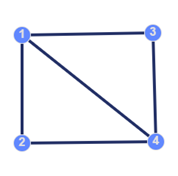
\includegraphics[width=0.17\textwidth]{imgs/Figura3}
    \caption{Exemplo de grafo simples\label{fig:imagem3}}
\end{figure}
\linebreak
- \underline{Multigrafo}, no caso de terem várias arestas a conectar os mesmos dois vértices, ou no caso de um vértice possuir um lacete, ou seja, uma “aresta” a ligar esse mesmo vértice nas duas extremidades.\\
\begin{figure}[h]
    \centering
    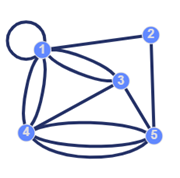
\includegraphics[width=0.17\textwidth]{imgs/Figura4}
    \caption{Exemplo de multigrafo com lacete\label{fig:imagem4}}
\end{figure}
\linebreak
\begin{flushright}{\scriptsize{(Nas companhias aéreas os passageiros detestam lacetes.\\O avião descola do aeroporto e pouco\\depois aterra no mesmo novamente!)}}\end{flushright}

\subsection{Digrafos ou grafos orientados}
São grafos que apresentam na sua totalidade arestas orientadas, mais conhecidas como arcos.\\

\begin{figure}[h]
    \centering
    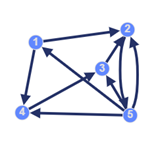
\includegraphics[width=0.2\textwidth]{imgs/Figura5}
    \caption{Exemplo de um digrafo, ou grafo orientado\label{fig:imagem5}}
\end{figure}

\subsection{Grafo Parcial e Subgrafo gerado de um dado grafo}
- \underline{Grafo Parcial}: Supressão de arestas, mantendo o número de vértices. Em contexto, podemos assumir 
que uma rota de voo é descontinuada por existir uma outra que implique escala ou por ser uma escala que já 
não faça sentido e exista uma outra rota direta para um dado destino.\\
%(o \linebreak faz com que a ultima linha do parágrafo ocupe a folha inteira)
\begin{figure}[h]
    \centering
    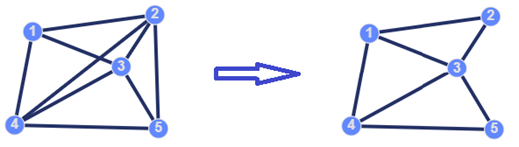
\includegraphics[width=0.2\textwidth]{imgs/Figura6}
    \caption{ À direita um grafo parcial resultante do grafo à esquerda com perda de arestas\label{fig:imagem6}}
\end{figure}
\linebreak
\indent - \underline{Subgrafo}: supressão de vértices e por consequência de todas as arestas com ligações a esses vértices. 
Em contexto, um destino deixa de servir os interesses da companhia, sendo canceladas como consequência 
todas as rotas para esse mesmo destino.
\linebreak
\begin{figure}[h]
    \centering
    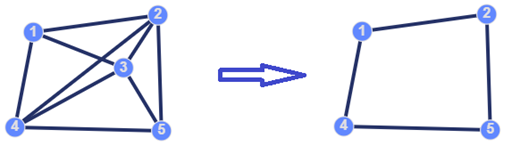
\includegraphics[width=0.2\textwidth]{imgs/Figura7}
    \caption{ À direita, subgrafo gerado do grafo à esquerda com perda de vértice e consequentes arestas ligadas\label{fig:imagem7}}
\end{figure}

\subsection{Grafo Subjacente e digrafo associado}
Quando queremos representar um Digrafo Associado a um dado grafo, na prática cada aresta ligada a 
dois vértices duplica, e as novas arestas passam a ter orientações opostas, aplicando-se o mesmo para os 
lacetes.\\
\indent Para representar um Grafo Subjacente a partir de um Digrafo, simplesmente tiramos as orientações aos 
arcos, tornando-se arestas paralelas e lacetes existentes desaparecem.\\
\indent Nas seguintes figuram podemos observar os conceitos de digrafo associado a um grafo e de grafo 
subjacente a um digrafo:\\

\begin{figure}[h]
    \centering
    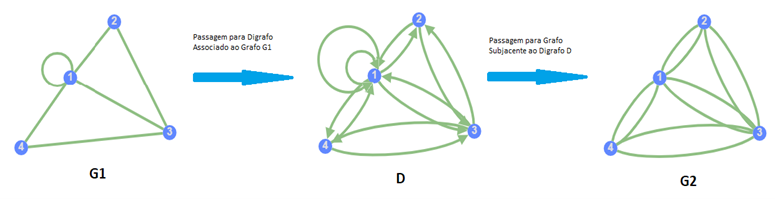
\includegraphics[width=0.2\textwidth]{imgs/Figura8}
    \caption{Transformação de um grafo no seu digrafo associado e consequente digrafo no seu grafo 
    subjacente
    \label{fig:imagem8}}
\end{figure}
\pagebreak
\subsection{ Cadeias e Ciclos}
Cadeias são uma sequência de arestas com início num dado vértice, tendo em comum numa extremidade 
o vértice que a precedeu e depois na outra extremidade o vértice da aresta adjacente seguinte. Podem 
dividir-se em:\\
\indent - \underline{Cadeia fechada}, tem início e fim no mesmo vértice;\\
\indent - \underline{Cadeia Simples}, não repete arestas;\\
\indent - \underline{Cadeia Elementar} , não repete vértices.\\
\indent - \underline{Ciclos} são cadeias simples fechadas.\\

\begin{figure}[h]
    \centering
    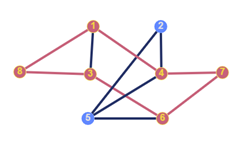
\includegraphics[width=0.2\textwidth]{imgs/Figura9}
    \caption{ Exemplo de um Ciclo, representado pelos vértices e arestas a vermelho\label{fig:imagem9}}
\end{figure}

\subsection{Caminhos e circuitos}
Caminhos seguem a mesma lógica das cadeias, com a diferença de respeitar a orientação das arestas, não 
se podendo ignorar o seu sentido, o que introduz algumas limitações:\\
\indent - \underline{Caminho fechado}, tem início e fim no mesmo vértice;\\
\indent - \underline{Caminho Simples}, não repete arestas;\\
\indent - \underline{Caminho Elementar}, não repete vértices.\\
\indent - \underline{Circuitos} são caminhos simples fechados.\\

\begin{figure}[h]
    \centering
    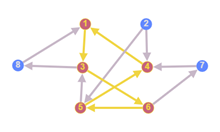
\includegraphics[width=0.2\textwidth]{imgs/Figura10}
    \caption{Exemplo de um Circuito, representado pelos arcos a amarelo
    \label{fig:imagem10}}
\end{figure}

\subsection{Graus dos vértices de um grafo}
Graus de um vértice v, define-se pelo número de arestas adjacentes a v. Define-se por deg(v), e por 
definição, o somatório dos graus de todos os vértices de um grafo é igual ao dobro do número de arestas 
desse mesmo grafo.\\
\indent Matematicamente traduz-se por  deg(V) = 2$\vert$E$\vert$, onde V simboliza todos os vértices e $\vert$E$\vert$ o número de 
arestas do grafo. No caso dos digrafos, ainda se aplica -> $deg(v) = deg^+(v) + deg^-(v)$, onde:\\
\indent - $deg^+(v)$ é o grau exterior de um digrafo, ou seja, o número de arestas onde o vértice v é a extremidade 
inicial;\\
\indent - $deg^-(v)$ é o grau interior de um digrafo, ou seja, o número de arestas onde o vértice v é a extremidade 
final.

\subsection{ Vizinhos de um vértice}
Diz-se que um vértice v é vizinho de um outro vértice u, se os dois estão ligados por uma aresta com 
extremidades nos dois vértices em questão.\\
\indent Define-se por $\Gamma(v)= \{ vizinho\_u1\,de\,v,\,vizinho\_u2\,de\,v,\,…\,,\,vizinho\_un\,de\,v \}$\\

$\Gamma^+(v)$ e $\Gamma^-(v)$ são também conceitos semelhantes no caso dos digrafos, com $\Gamma^+(v)$ sendo os sucessores de v e $\Gamma^-(v)$ os antecessores de v.
